% !TeX root = ../main.tex

\section{Análisis de resultados}

\subsection{Datos sintéticos}
Para empezar, trabajamos con unos datos sintéticos que simulan una zona del Sol en calma. El formato de estos datos es $[101,\,4,\,336,\,336]$, lo que significa que tenemos $101$ longitudes de onda, las $4$ componentes de Stokes ($I$, $Q$, $U$ y $V$) y un tamaño espacial de $336\times336$ píxeles. \\
Para poner a prueba los métodos de deconvolución, el primer paso fue emborronar artificialmente estas imágenes usando una PSF de tipo Airy. Esta función es una aproximación teórica de cómo se comporta un telescopio ideal cuya única limitación es tener una apertura circular. Matemáticamente, su perfil radial se escribe así:
\begin{equation}
    \label{eq:PSF}
    PSF(r) = I_0 \left(\frac{2 J_1(kr)}{kr} \right)
\end{equation}

donde $J_1$ es la función de Bessel de primer orden, $k$ es una constante que depende del diámetro del telescopio y de la longitud de onda, e $I_0$ es la intensidad máxima. 

En este caso se usa una PSF de 30 pixeles de radio y un tamaño de bulbo central de 3 pixeles, donde su representación visual es la siguiente:

\begin{figure}[H]
    \centering
    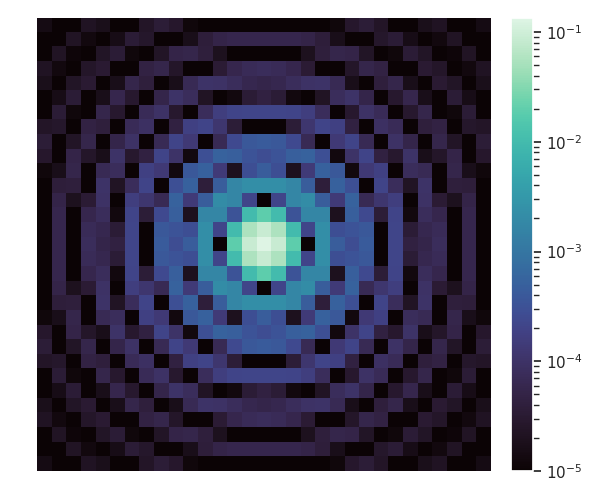
\includegraphics[width=0.7\textwidth]{img/comparacion_intensidad_4_psf.png}
    \caption{Esta imagen muestra la PSF de tipo Airy utilizada para emborronar la imagen original. Se puede observar que el bulbo central tiene un tamaño de 3 píxeles y que el radio de la PSF es de 30 píxeles. Esta representada en escala logaritmica para poder observar mejor la caída de la intensidad en los anillos de difracción.}
    \label{fig:psfAiry}
\end{figure}

Obviamente, para que la simulación sea realista, también necesitamos meter ruido en la ecuación. Añadimos ruido blanco gaussiano a cada componente de Stokes. Pero como la señal en el canal $I$ es muchísimo más fuerte que en el canal $V$, tuvimos que aplicar un esquema de ruido relativo. Esto significa que la desviación estándar ($\sigma$) del ruido se define como un porcentaje $p$ de la amplitud máxima de cada señal en particular, imitando mejor lo que ocurre en una observación real:
\begin{equation}
    I_{max} = \max(I(\mathbf{x})), \quad V_{max} = \max(|V(\mathbf{x})|)
\end{equation}
donde $\mathbf{x}$ representa las coordenadas espaciales y espectrales del cubo de datos. A partir de estos máximos, las desviaciones estándar para un porcentaje de ruido $p$ se definen como:
\begin{equation}
    \sigma_I = I_{max} \cdot \frac{p}{100}, \quad \sigma_V = V_{max} \cdot \frac{p}{100}
\end{equation}


\subsubsection{Análisis de los distintos métodos de deconvolución: Fourier, Wiener y Richardson-Lucy}

Primero se realizará una comparación visual entre los distintos métodos de deconvolución a partir de la Intensidad (primera componente de Stokes). Escogeremos una longitud de onda arbitraria y la emborronoramos con un ruido del $0.1 \%$. El resultado es el siguiente.



\begin{figure}[H]
    \centering
    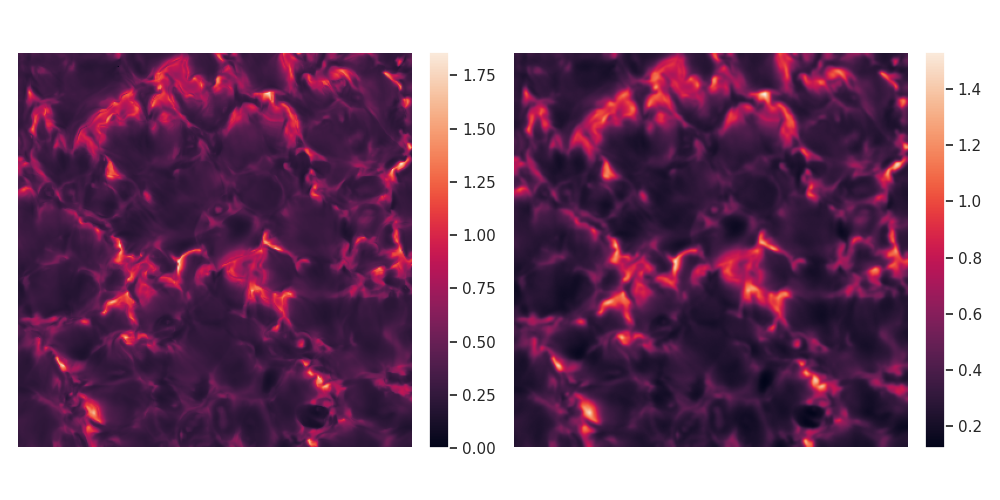
\includegraphics[width=0.9\textwidth]{img/comparacion_intensidad_1_original_borrosa.png}
    \caption{Esta imagen muestra dos mapas de intensidad. A la izquierda se muestra el mapar sintético original, mientras que a la derecha se muestra el mapa convolucionado con la PSF (\ref{fig:psfAiry}) y con un ruido del $0.1 \%$. Se puede observar que la imagen de la derecha está emborronada y que se han perdido detalles finos de la imagen original.}
    \label{fig:intensidadSintEmborro}
\end{figure}

Aunque se ve el emborronamiento, nos centraremos en una zona concreta de la imagen para observar mejor los detalles. Está representada en la siguiente figura:

\begin{figure}[H]
    \centering
    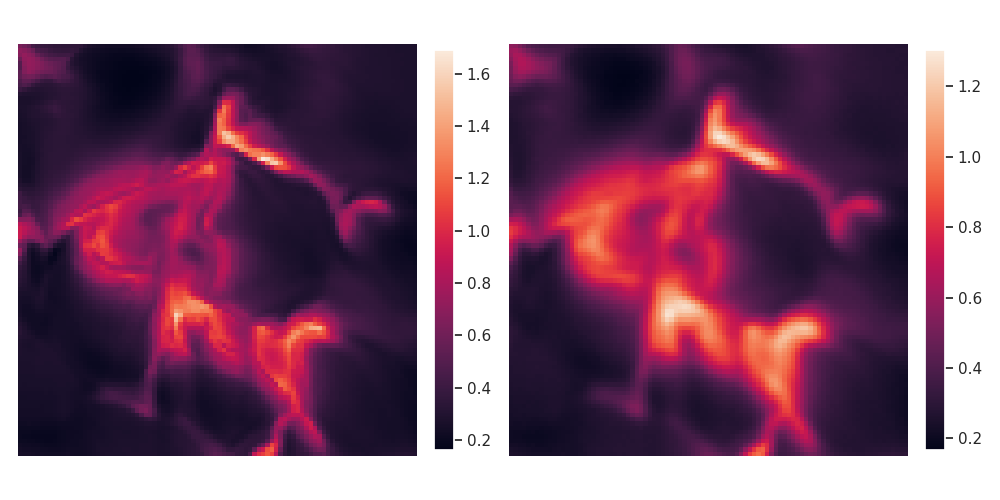
\includegraphics[width=0.9\textwidth]{img/comparacion_intensidad_5_original_borrosa_zoom.png}
    \caption{Región de la imagen de la figura \ref{fig:intensidadSintEmborro} donde se puede observar mejor el emborronamiento de la imagen. A la izquierda se muestra el mapa sintético original, mientras que a la derecha se muestra el mapa convolucionado con la PSF (\ref{fig:psfAiry}) y con un ruido del $0.1 \%$.}
    \label{fig:intensidadSintEmborroZoom}
\end{figure}

Entonces realizamos la deconvolución con los distintos métodos (Wiener, Fourier, Richardson-Lucy) y comparamos visualmente los resultados. El resultado es el siguiente:

\begin{figure}[H]
    \centering
    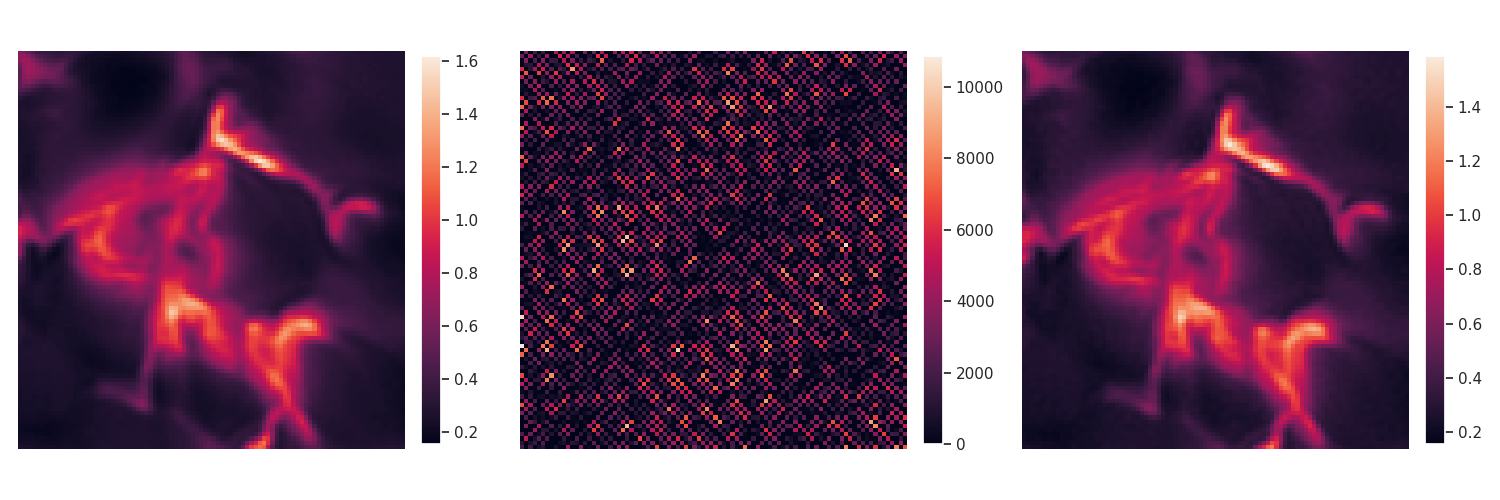
\includegraphics[width=1.0\textwidth]{img/comparacion_intensidad_6_deconvoluciones_zoom.png}
    \caption{Resultados de la deconvolución con los distintos métodos. A la izquierda se encuentra el mapa deconvolucionado con el método de Wiener, en el centro se encuentra el mapa deconvolucionado con el método de Fourier y a la derecha se encuentra el mapa deconvolucionado con el método de Richardson-Lucy.}
    \label{fig:deconvolucionClasicaZoom}
\end{figure}

Y si miramos los resultados de las métricas RMSE y SSIM, obtenemos los siguientes resultados:

\begin{figure}[H]
    \centering
    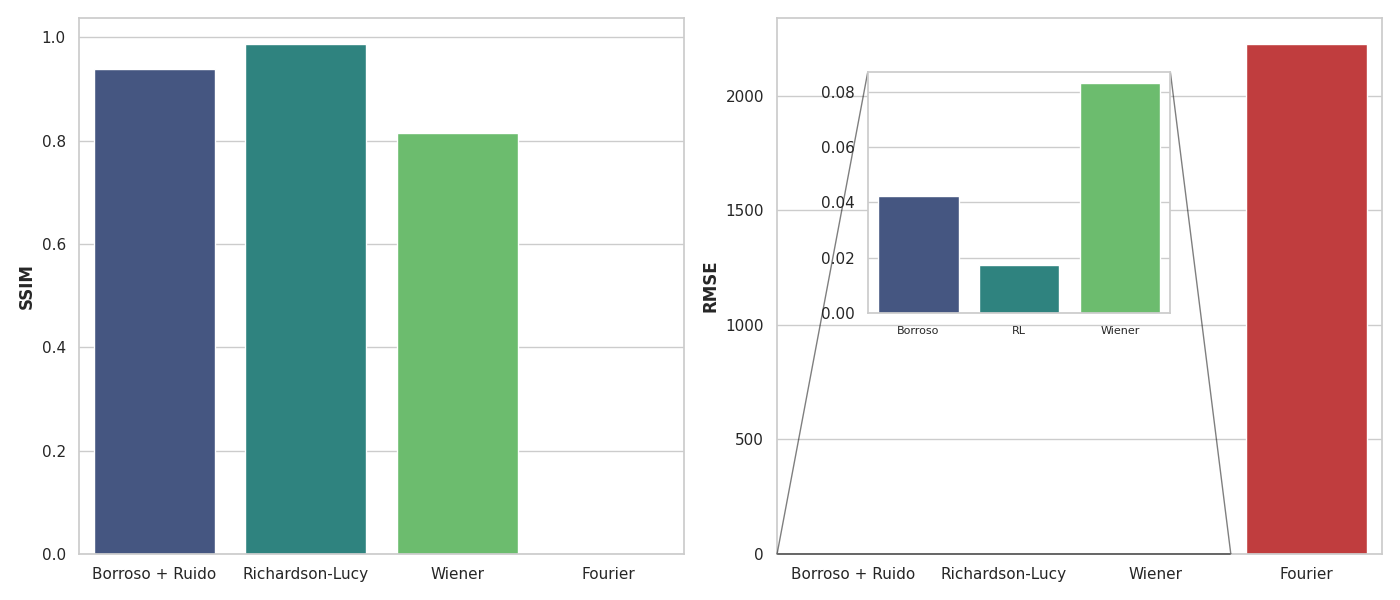
\includegraphics[width=1.0\textwidth]{img/comparacion_intensidad_3_barras.png}
    \caption{Valores de las métricas SSIM (izquierda) y RMSE (derecha) para los diferentes métodos de deconvolución. Se añade también la imagen emborronada para comparar sus valores. Debido al elevado valor de RMSE obtenido con el método de Fourier, la gráfica de la derecha incorpora una ampliación que permite apreciar con mayor detalle las diferencias entre el resto de métodos.}
    \label{fig:rsmeSsimIntensidad}
\end{figure}

Empezando por el método de Fourier, salta a la vista que sus métricas son desastrosas: tiene un SSIM casi nulo y un RMSE altísimo. Físicamente, esto se traduce en una imagen donde se ha perdido absolutamente todo el detalle. Como ya habíamos anticipado teóricamente, este método no soporta nada bien el ruido, quedando claro que no nos sirve para imágenes reales que no sean perfectas.

Si pasamos al filtro de Wiener, la situación es engañosa. Visualmente da la sensación de haber recuperado bastante detalle, pero si miramos los números, el SSIM es más bajo y el RMSE es más alto que los de la propia imagen emborronada sin tocar. Es decir, aunque a ojo parezca mejor, la reconstrucción real es peor. Seguramente esto pase porque hemos utilizado la versión más básica del filtro de Wiener; en la literatura actual hay versiones mucho más sofisticadas que logran corregir estos fallos (por ejemplo, \cite{orieuxBayesianEstimationRegularization2010}).

Por el contrario, el algoritmo de Richardson-Lucy es el claro ganador de esta comparativa. Consigue mejorar el SSIM y bajar el RMSE respecto a la imagen borrosa de partida. Demuestra ser mucho más robusto frente al ruido, y si miramos el resultado, es evidente cómo logra rescatar detalles finos que se habían emborronado por culpa de la PSF.

\subsubsection{Problema de la deconvolución de V}
Si analizamos como evoluciona la deconvolución de la señal de Stokes $V$, y lo analizamos a distintos porcentajes de ruido, obtenemos los siguientes resultados:

\begin{figure}[H]
    \centering
    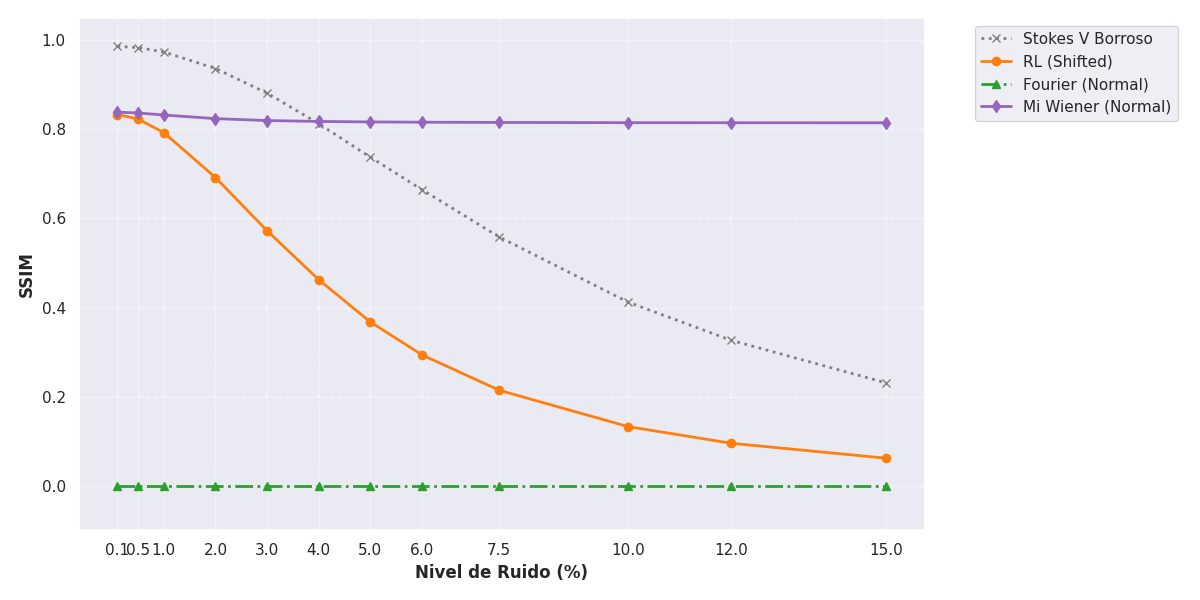
\includegraphics[width=1.0\textwidth]{img/experimento_stokesV_3_comparativa_shift.png}
    \caption{Evolución del SSIM en función del nivel de ruido para distintos métodos de deconvolución aplicados a la componente Stokes V. Se comparan los resultados de la imagen borrosa original frente a Richardson-Lucy (con \textit{shift} positivo), el filtro de Fourier y el filtro de Wiener.}
    \label{fig:SSIM_frenteARuidoV}
\end{figure}

Como la componente de Stokes $V$ tiene una amplitud tan pequeña, resulta extremadamente sensible al ruido. Esto provoca que ninguno de los algoritmos clásicos de deconvolución sea capaz de recuperar la señal original de forma satisfactoria. El método que ofrece mejores resultados es el filtro de Wiener. Para ilustrar este efecto, a continuación se muestra el mapa bidimensional recuperado por este filtro con un ruido del 2%:


\begin{figure}[H]
    \centering
    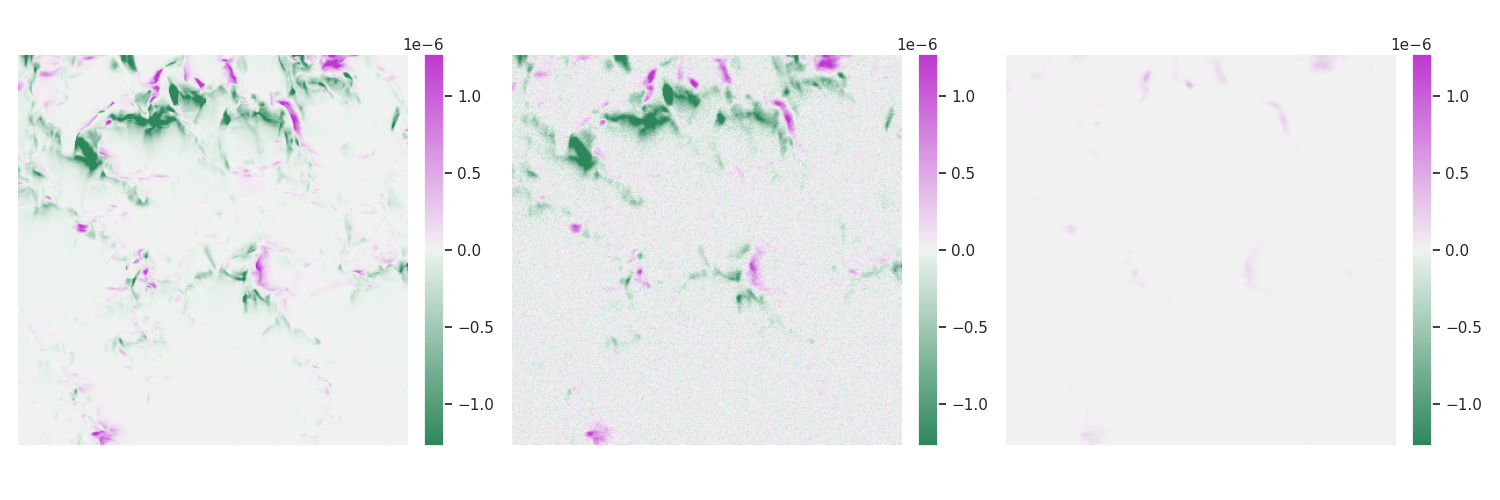
\includegraphics[width=1.0\textwidth]{img/experimento_stokesV_2_visualizacion.png}
    \caption{Comparativa visual de la componente Stokes V. De izquierda a derecha: mapa original (Ground Truth), mapa degradado con un $2\%$ de ruido, y resultado tras la deconvolución mediante el filtro de Wiener, mostrando el sobre-suavizado de la señal.}
    \label{fig:visualizacionStokesV}
\end{figure}

Esto explica por qué el índice SSIM se mantiene constante: el filtro de Wiener consigue eliminar el ruido, pero no logra recuperar la estructura de la señal original y termina suavizándola demasiado. 

Por lo tanto, este análisis demuestra que es inviable deconvolucionar la señal de Stokes $V$ con los métodos clásicos. Por esta razón, en este TFG se utiliza el método desarrollado para calcular el campo magnético directamente, evitando tener que deconvolucionar la señal de Stokes $V$.


\subsubsection{Método adaptado de Van Noort}
Antes de ver imágenes, vamos a comprobar si nuestro método converge como debería. Para ello, preparamos los datos igual que en el caso anterior: convolucionamos con la PSF y le metemos ruido. Como nuestra técnica es iterativa, va resolviendo el sistema poco a poco en cada paso. La mejor forma de asegurarnos de que todo marcha bien es vigilar el "residuo" tras cada iteración.

Ese residuo no es más que la diferencia entre lo que esperábamos obtener y la aproximación que ha logrado calcular el algoritmo en ese momento. Si medimos este error total (calculando la norma euclidiana $L_2$), obtenemos lo que llamamos diferencia iterativa. En la gráfica de abajo hemos representado esta evolución poniendo el eje vertical en escala logarítmica, lo que ayuda a ver muy claro cómo el error se desploma:

\begin{figure}[H]
    \centering
    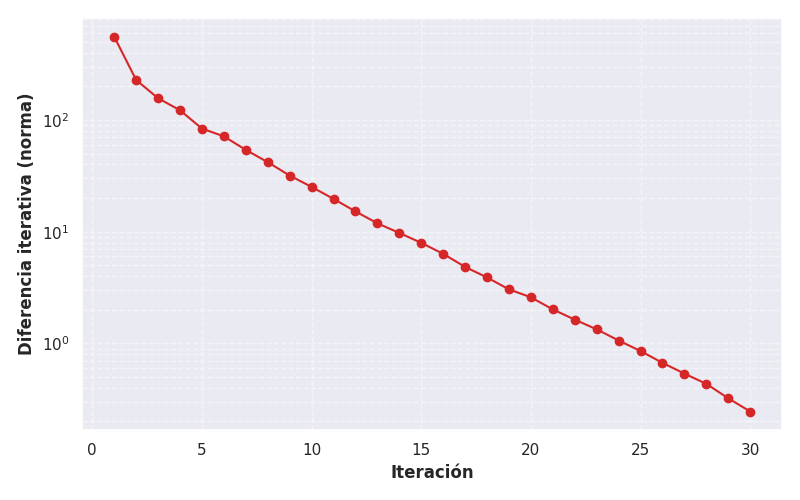
\includegraphics[width=0.8\textwidth]{img/experimento_noor_1_convergencia.png}
    \caption{Esta imagen muestra la evolución de la diferencia iterativa (la norma del residuo) a lo largo de las iteraciones del algoritmo de Noor. Se puede observar cómo el error va disminuyendo progresivamente, lo que indica que el método converge de forma correcta.}
    \label{fig:convergenciaNoor}
\end{figure}

Veremos entonces el resultado de esta deconvolución:

\begin{figure}[H]
    \centering
    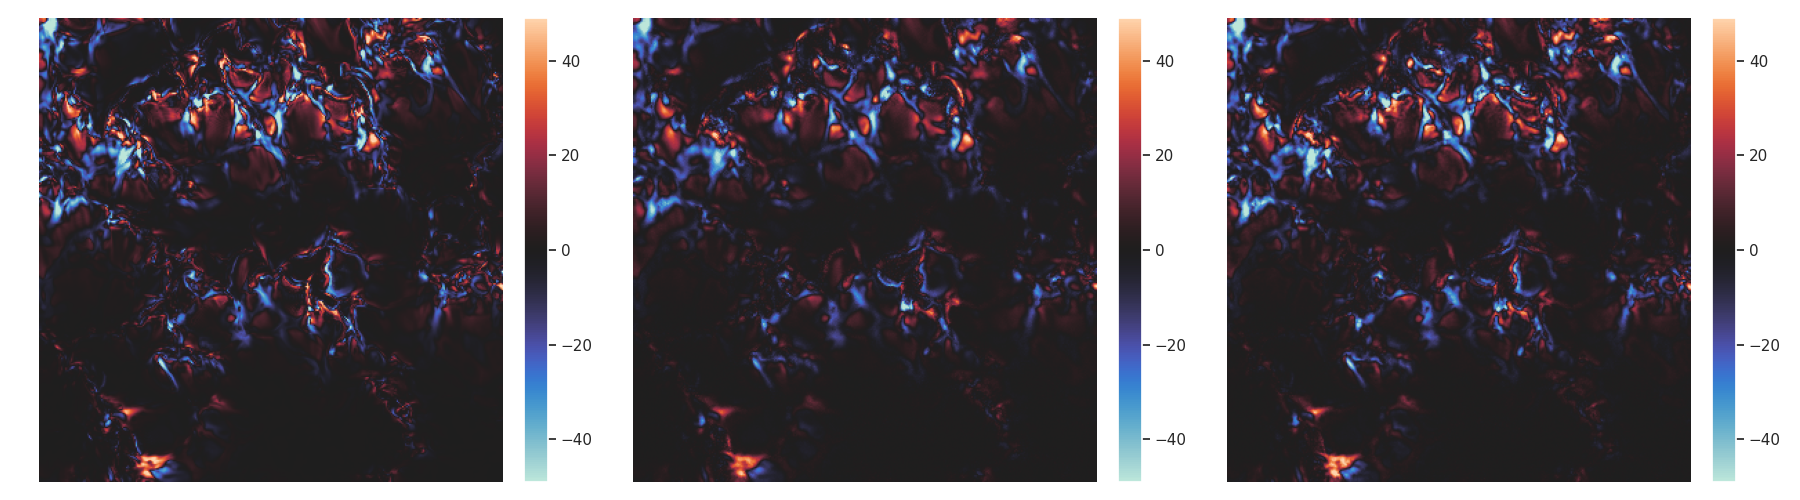
\includegraphics[width=1.0\textwidth]{img/experimento_noor_2_comparativa_b copy.png}
    \caption{Comparativa visual del campo magnético, representado en Gauss. De izquierda a derecha: mapa original (Ground Truth), mapa degradado con ruido, y resultado tras la deconvolución mediante el método adaptado de Noor.}
    \label{fig:campoMagDeco}
\end{figure}

Igual que antes, volveremos a hacer zoom a la misma zona de interes para observar mejor los detalles de la imagen. El resultado es el siguiente:

\begin{figure}[H]
    \centering
    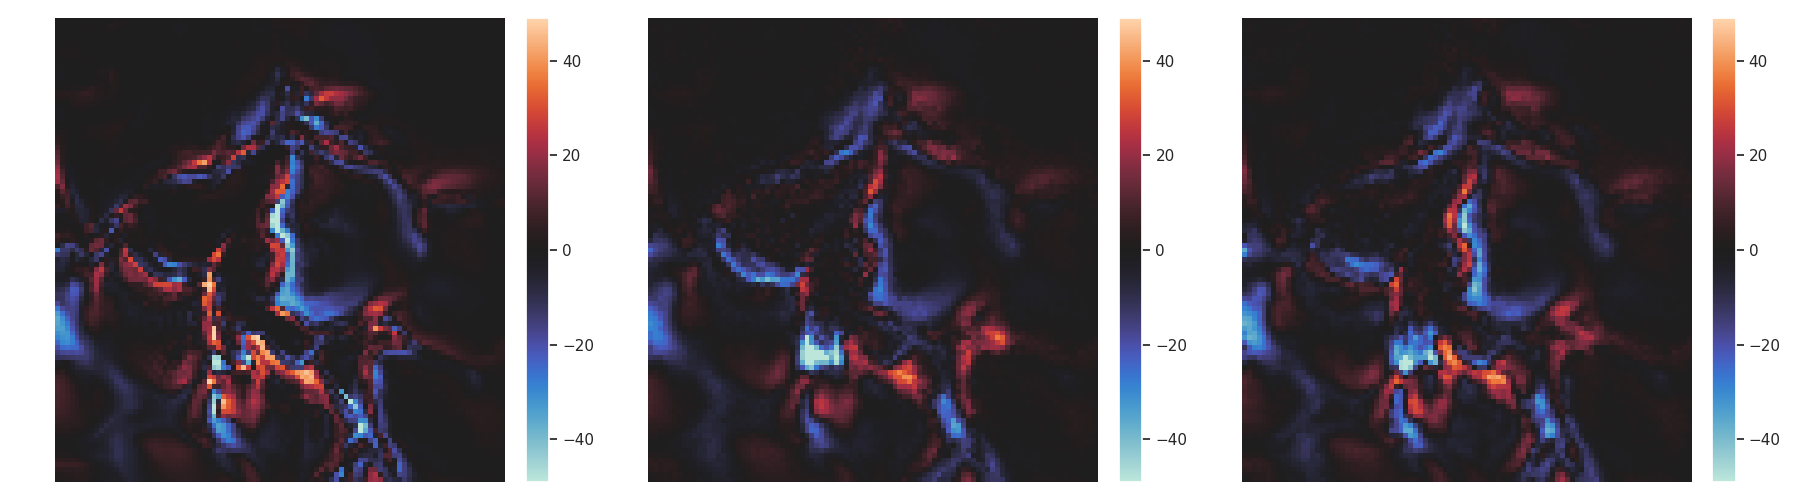
\includegraphics[width=1.0\textwidth]{img/experimento_noor_2b_comparativa_b_zoom.png}
    \caption{Comparativa visual del campo magnético, representado en Gauss. De izquierda a derecha: mapa original (Ground Truth), mapa degradado con ruido, y resultado tras la deconvolución mediante el método adaptado de Noor. Se puede observar que el método logra recuperar detalles finos del campo magnético que se habían perdido en la imagen degradada.}
    \label{fig:campoMagDecoZoom}
\end{figure}

Como salta a la vista, nuestro método consigue rescatar la estructura original del campo magnético. Las zonas vuelven a estar definidas e incluso recuperamos picos de intensidad que el emborronamiento se había "comido", lo cual es todo un éxito. Sí que es cierto que hay ciertos bulbos magnéticos que no quedan perfectos, pero es totalmente esperable: al emborronar la imagen físicamente perdimos parte de la información original, por lo que ningún método podrá inventársela. Salvando ese detalle, el resultado general es estupendo y confirma que nuestra técnica sí es capaz de extraer el campo magnético combinando las señales $I$ y $V$. 

Si miramos un mapa de diferencias entre la imagen original y borrosa, y la imagen original y la deconvolucionada, obtenemos el siguiente resultado:

\begin{figure}[H]
    \centering
    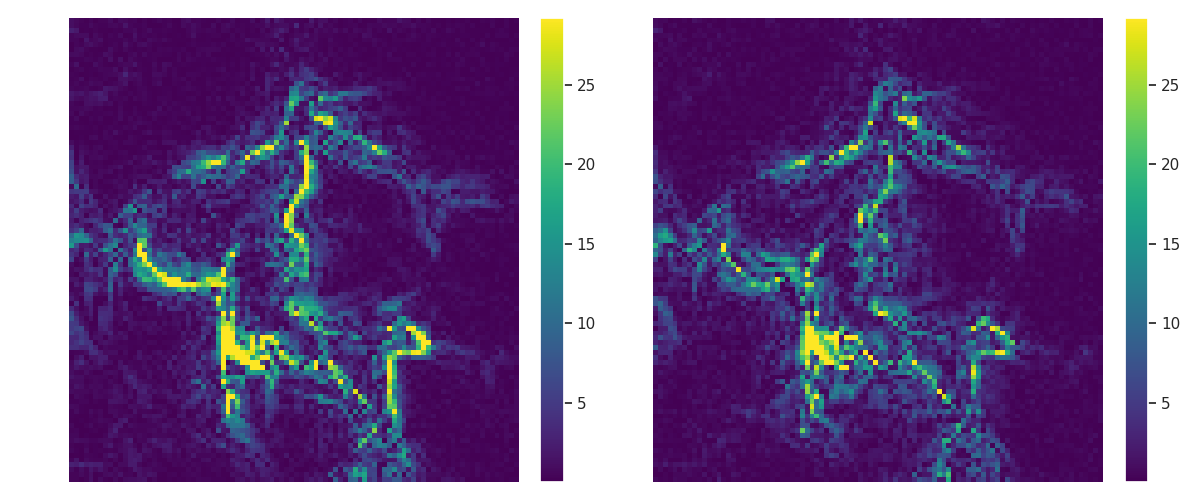
\includegraphics[width=1.0\textwidth]{img/experimento_noor_3b_residuos_zoom.png}
    \caption{Mapa de diferencias entre la imagen original y la degradada, y la imagen original y la deconvolucionada.}
    \label{fig:diferenciasZoom}
\end{figure}

Como vemos en la gráfica de diferencias, el residuo baja significativamente en las zonas de los filamentos, lo que demuestra que realmente está reconstruyendo la estructura. \\
Esta mejora que vemos a simple vista también la confirman los números. Nuestra imagen emborronada de partida tenía un SSIM de $0.8401$ y un RMSE de $5.2568$. Después de pasarle nuestro método adaptado de Van Noort (usando regularización de Laplace), el SSIM sube a $0.8575$ y el RMSE cae a $4.6995$. Matemáticamente, nos hemos acercado bastante más a la imagen ideal.

El siguiente paso natural es ver qué tal se porta el algoritmo cuando cambiamos los niveles de ruido. Hay que tener en cuenta que este método es bastante sensible al número de iteraciones: si nos pasamos dando pasos, acabaremos sobreajustando la señal y amplificando el ruido. El reto aquí es dar con el equilibrio perfecto entre cuántas iteraciones damos y cuánto ruido tiene la imagen. 

Para ello se realizó un estudio donde se encuentra el mejor SSIM y RMSE para distintos niveles de ruido, variando el número de iteraciones. Si vemos el mejor SSIM frente al nivel de ruido, obtenemos el siguiente resultado:

\begin{figure}[H]
    \centering
    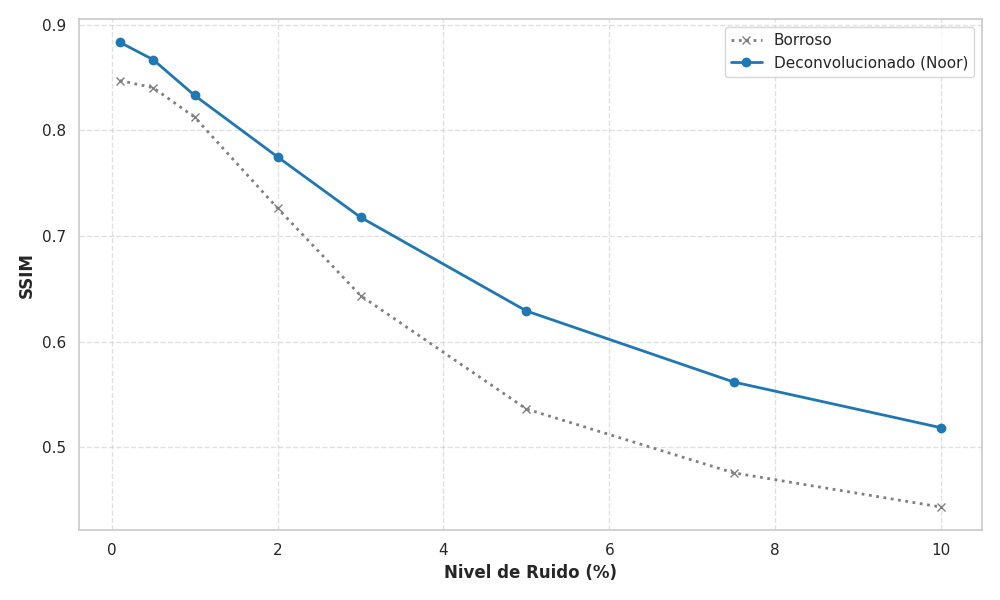
\includegraphics[width=0.7\textwidth]{img/experimento_noor_4_limite_ruido.png}
    \caption{Evolución del SSIM frente al nivel de ruido para el método adaptado de Noor. Se observa que el método siempre logra mejorar la imagen original.}
    \label{fig:SSIMfrenteARuidoNoor}
\end{figure}

Y si presentamos el mejor RMSE frente al nivel de ruido, obtenemos el siguiente resultado:

\begin{figure}[H]
    \centering
    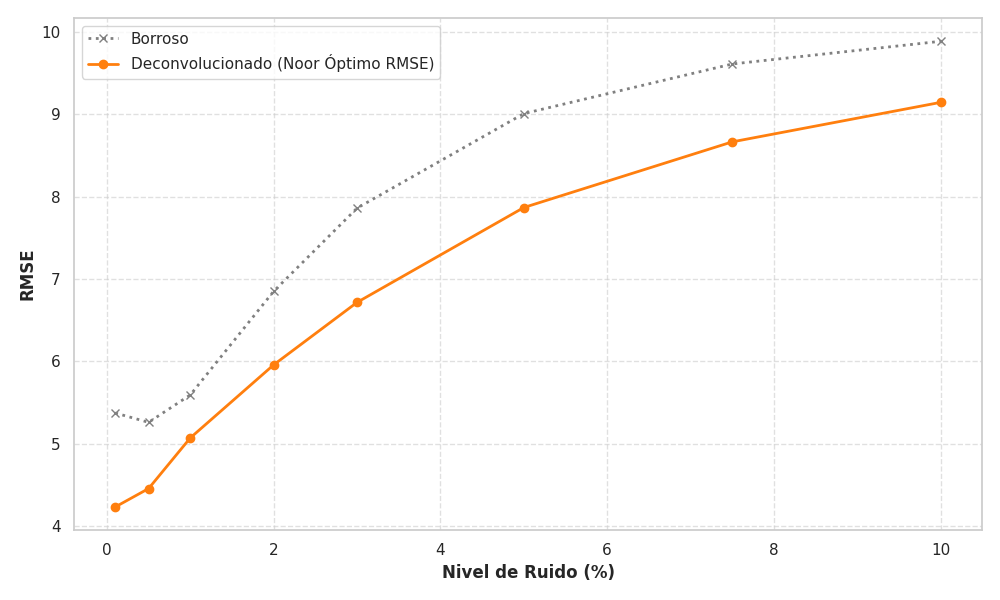
\includegraphics[width=0.7\textwidth]{img/experimento_noor_4b_limite_ruido_rmse.png}
    \caption{Evolución del RMSE frente al nivel de ruido para el método adaptado de Noor. Se observa que siempre es inferior.}
    \label{fig:RMSEfrenteARuidoNoor}
\end{figure}

Lo interesante de estas gráficas es ver que, sin importar cuánto ruido le echemos, el método siempre logra mejorar la imagen de partida. La clave de esto es que nuestro algoritmo no trabaja a ciegas; se apoya directamente en la física del problema para buscar una solución que encaje con la ecuación de transferencia radiativa. Gracias a esta restricción física, el método siempre es capaz de rascar algo de la señal original por mucho ruido que haya de fondo.

Si nos fijamos ahora en cuántas iteraciones hacen falta para dar con el mejor resultado en cada caso, llegamos a la siguiente gráfica:

\begin{figure}[H]
    \centering
    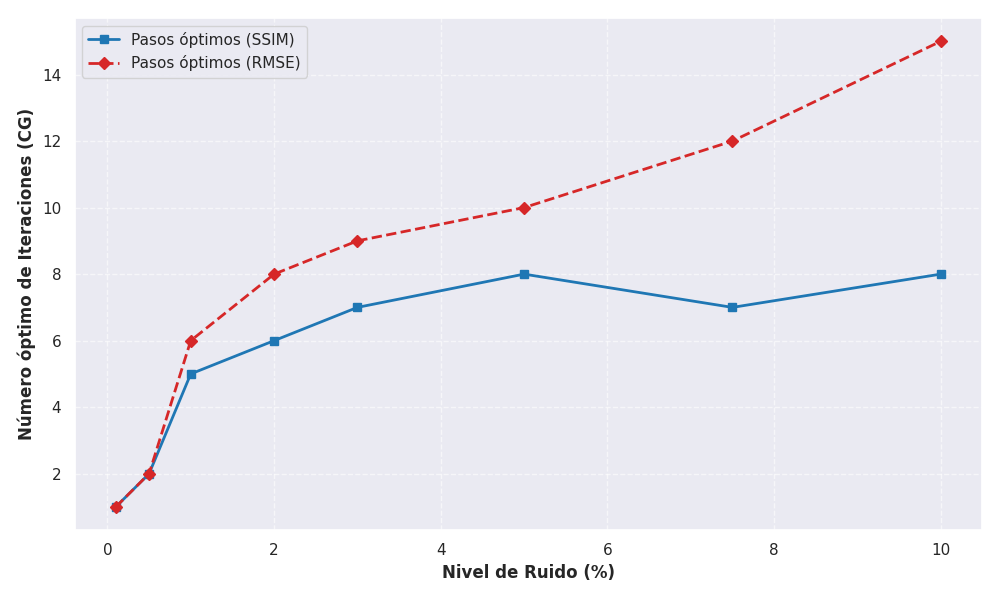
\includegraphics[width=0.7\textwidth]{img/experimento_noor_5_limite_ruido_pasos.png}
    \caption{Evolución del número de iteraciones frente al nivel de ruido para el método adaptado de Noor. La curva roja representa el numero de iteraciones para el valor de RMSE, y la curva azul representa el número de iteraciones para el valor de SSIM. Se observa que a medida que aumenta el nivel de ruido, se necesitan más iteraciones para conseguir el mejor resultado.}
    \label{fig:pasosfrenteARuidoNoor}
\end{figure}

Salta a la vista que siempre hacen falta más iteraciones para minimizar el RMSE que para alcanzar el mejor SSIM. Básicamente, el algoritmo necesita seguir iterando un rato más para limpiar el ruido estadístico (lo que mejora el RMSE), pero al hacerlo llega a un punto en el que empieza a emborronar ligeramente la estructura (lo que empeora el SSIM). Es el típico compromiso entre matar el ruido y conservar los bordes nítidos, algo parecido a lo que le pasaba a la componente $V$ en la figura (\ref{fig:visualizacionStokesV}).

\subsection{Datos reales} \label{sec:datosReales}
Ha llegado el momento de la verdad: probar todo esto con datos reales. Para ello, utilizamos las observaciones del experimento Sunrise-TUMAG disponibles públicamente \cite{SUNRISETuMagTUMAGData}. Concretamente, hemos cargado el archivo 
\begin{itemize}
    \item \textit{01\_QSUN\_TM\_00\_Mg1\_10\_10072024T131604\_LV\_1.0\_v0.4.fits}
\end{itemize}

Su estructura interna es $[10,\,4,\,1600,\,1600]$, lo que se traduce en 10 puntos de longitud de onda distintos, las 4 componentes de Stokes, y un mapa espacial enorme de $1600\times1600$ píxeles. 

El PSF fue cedido por el equipo de óptica de la sección de  física solar del IAA. Esta PSF se consiguió modelando computacionalmente la óptica del telescopio Sunrise, y se puede observar en la siguiente figura:

\begin{figure}[H]
    \centering
    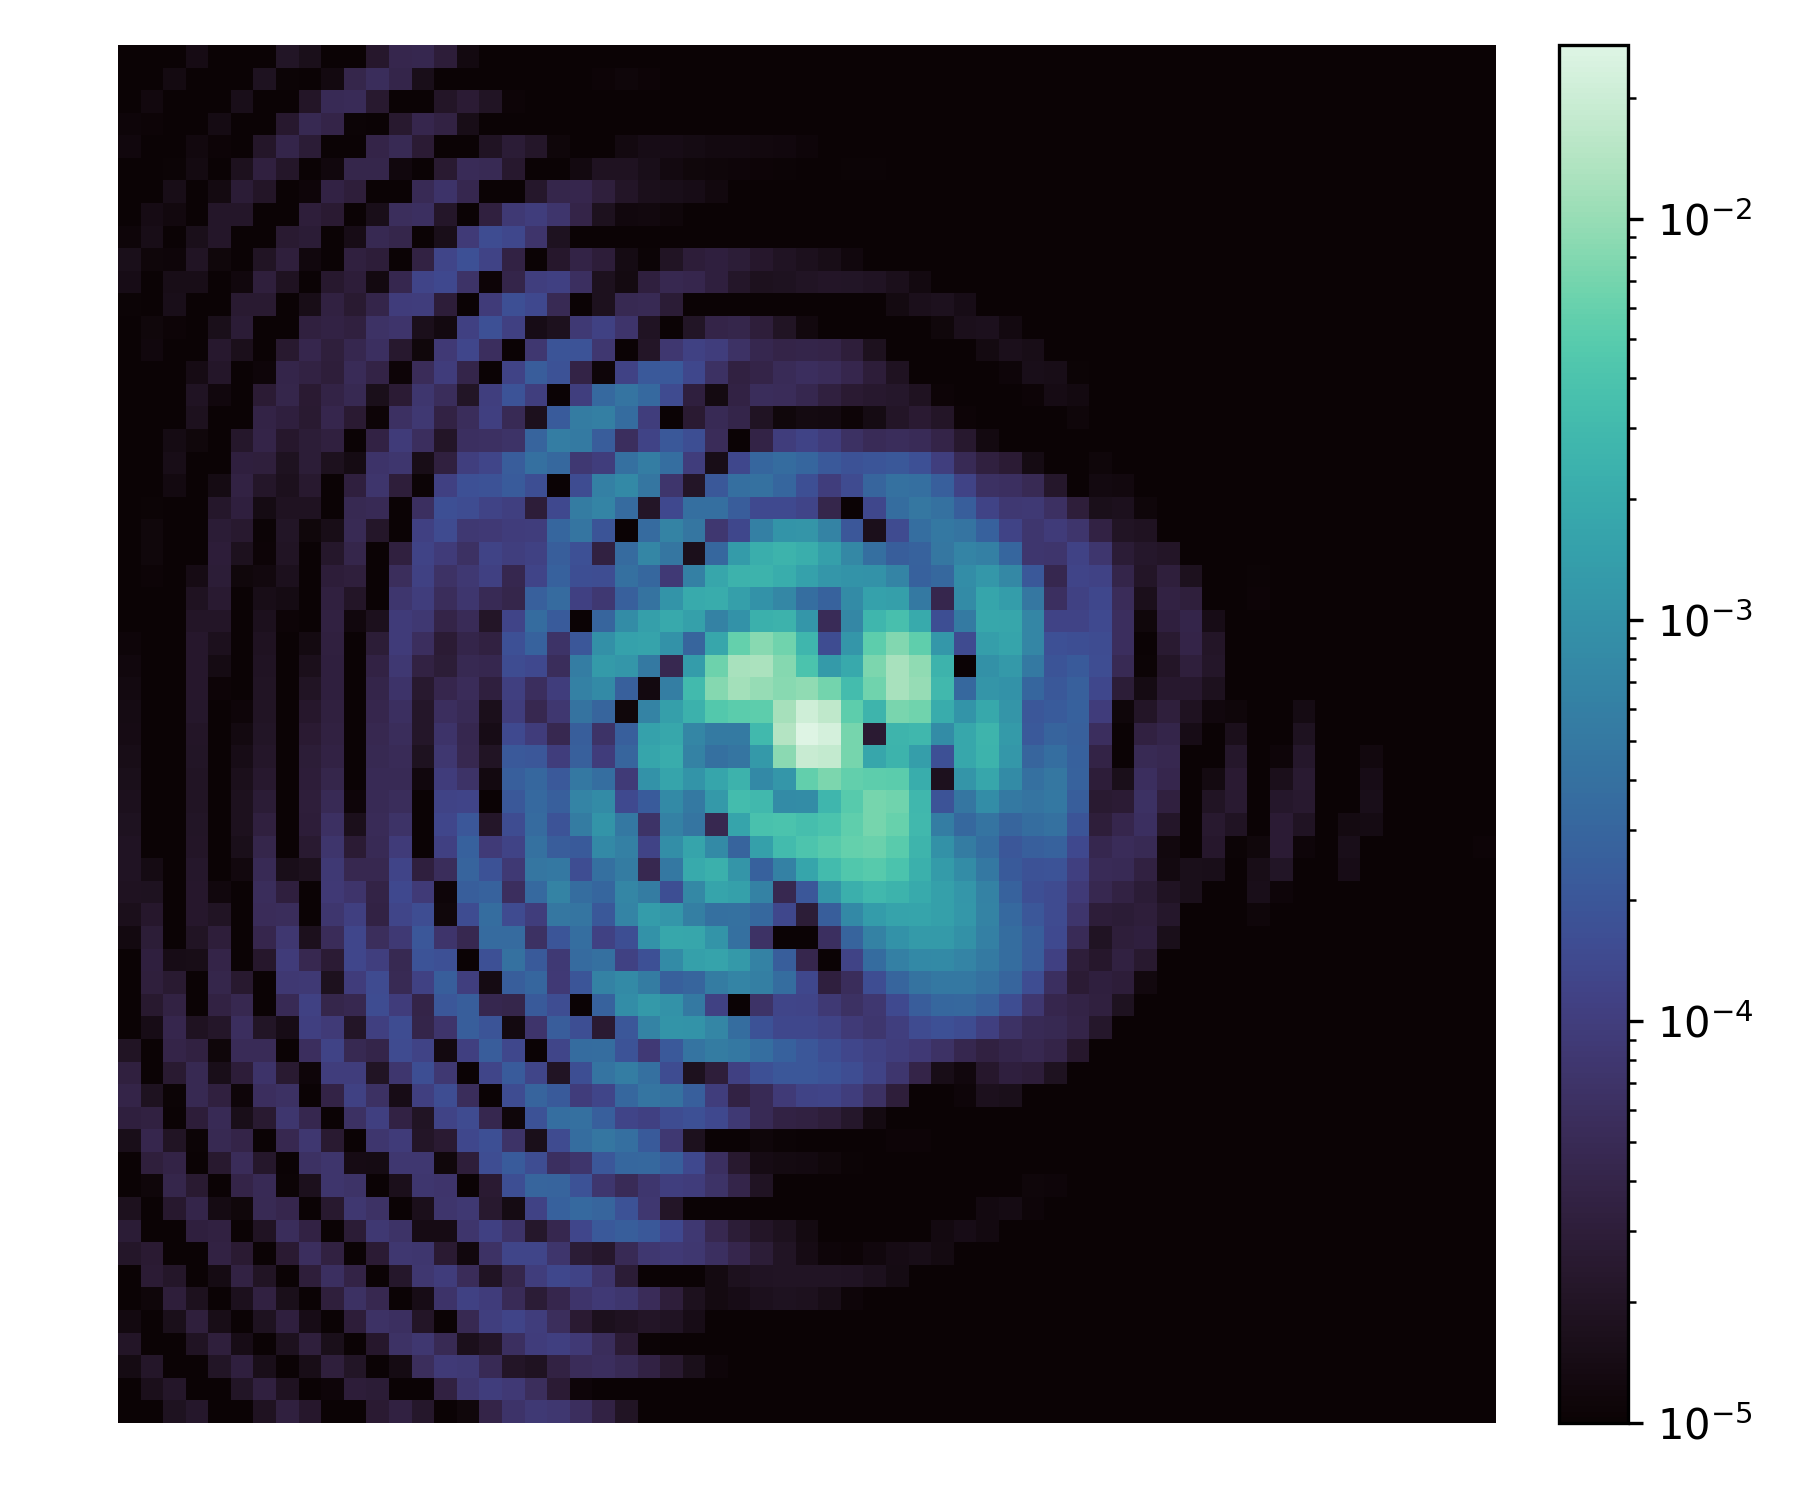
\includegraphics[width=0.7\textwidth]{img/exp4_4_psf.png}
    \caption{Esta imagen muestra la PSF del telescopio Sunrise. Se muestra en escala logaritmica para poder observar mejor la caída de la intensidad en los anillos de difracción.}
    \label{fig:psfReal}
\end{figure}


\subsubsection{Algoritmo de Richarson-Lucy}

Entonces, al igual que antes, cogemos una longitud de onda arbitraria y realizamos la deconvolución con el método de Richardson-Lucy. El resultado es el siguiente:

\begin{figure}[H]
    \centering
    \includegraphics[width=0.9\textwidth]{img/exp4_1_intensidad.png}
    \caption{Intensidad de la imagen deconvolucionada con el método de Richardson-Lucy. En la parte izquierda se muestra la imagen original, mientras que en la parte derecha se muestra la imagen deconvolucionada. Se puede observar que la imagen deconvolucionada tiene más detalle y contraste que la imagen original.}
    \label{fig:intensidadDecoReal}
\end{figure}

Visualmente ya se nota que Richardson-Lucy hace bien su trabajo. Rescata detalles de la imagen que antes estaban difuminados y le da un "empujón" importante al contraste general. 

El problema ahora a la hora de medir esta mejora es que estamos ante datos reales: no existe una "imagen ideal" con la que compararnos, así que las métricas SSIM y RMSE ya no nos sirven. Para sortear esto, tiramos de la métrica RMS (\textit{Contraste Cuadrático Medio}), que simplemente mide el contraste interno de la imagen:
\begin{equation}
    RMS = \sqrt{\frac{1}{N} \sum_{i=1}^{N} (I_i - \bar{I})^2}
\end{equation}

La lógica aquí es sencilla: a mayor RMS, más contraste y, en principio, más detalle fino habremos recuperado. En números, pasamos de un RMS inicial de $0.2028$ a $0.2193$ tras la deconvolución. Es una subida del $8.2\%$, lo que confirma numéricamente la mejora en contraste que ya apreciábamos a simple vista.

\subsubsection{Medición del campo magnético}
Ahora mediremos el algoritmo de Noor para medir el campo magnético a partir de la señal de Stokes $I$ y $V$. Para observar mejor los resultados, observaremos una región de interés de la imagen, que es la siguiente tras deconvolucionarlo con el algoritmo:

\begin{figure}[H]
    \centering
    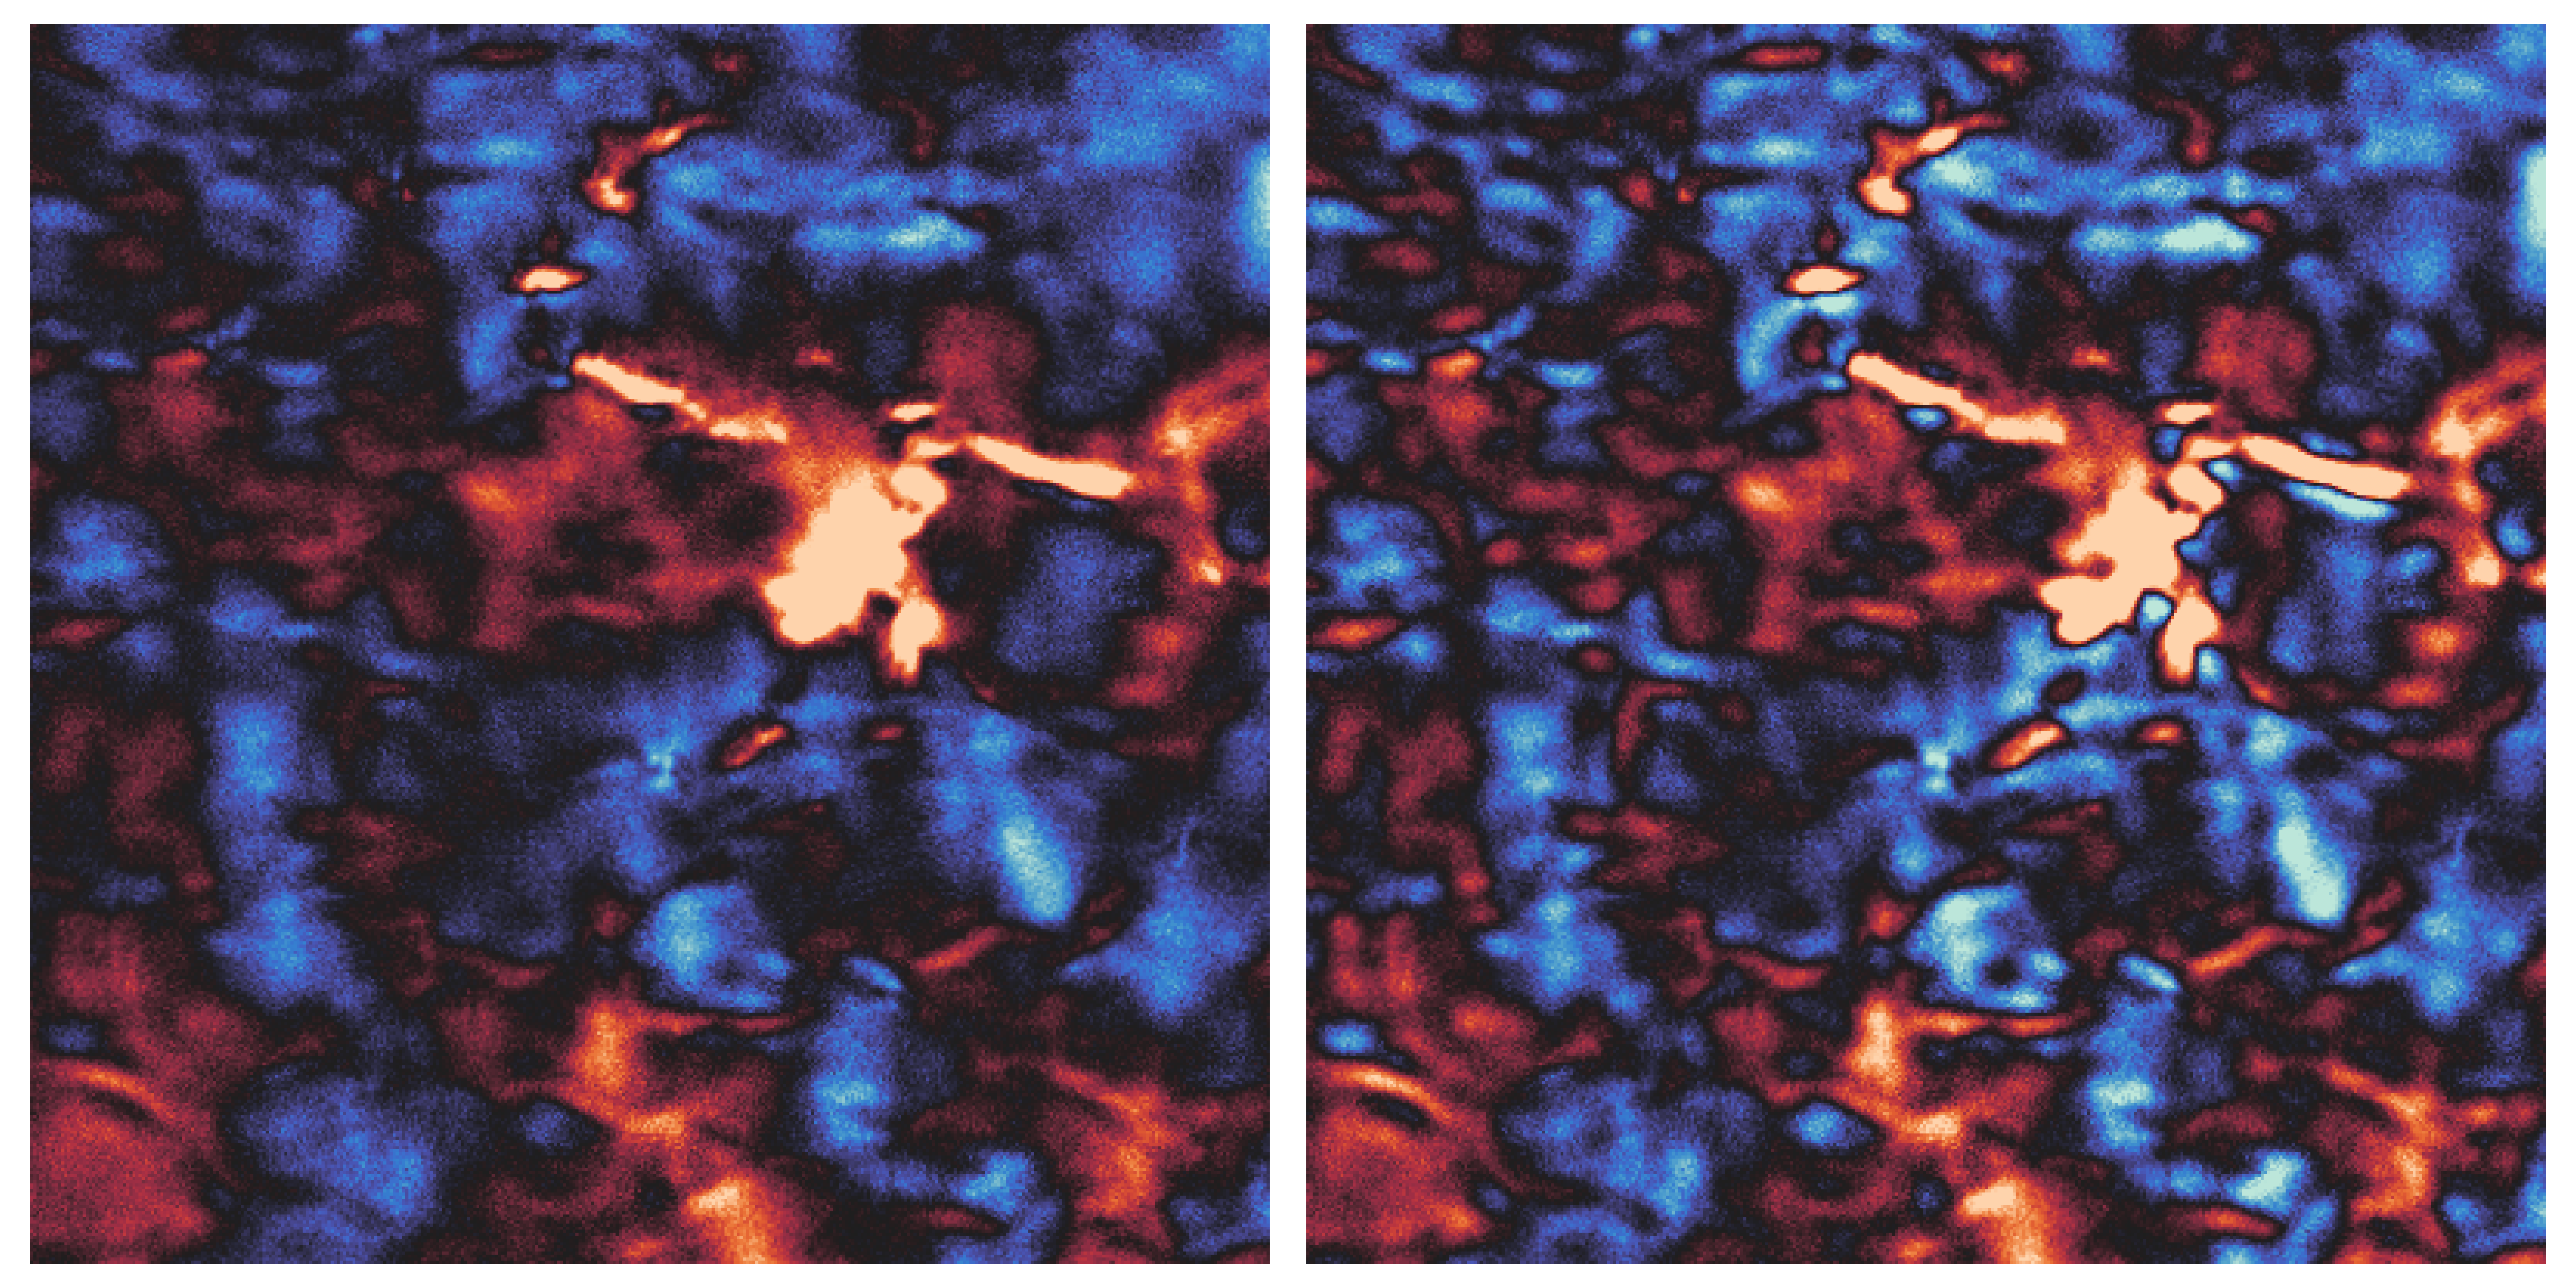
\includegraphics[width=0.9\textwidth]{img/exp4_3_campoB_zoom.png}
    \caption{Campo magnético medido a partir de la señal de Stokes $I$ y $V$ mediante el método adaptado de Noor. Se observa que el campo magnético tiene una estructura más definida y detallada que la imagen original.}
    \label{fig:campoMagDecoReal}
\end{figure}

Al igual que antes, se observa que el método logra recuperar la estructura del campo magnético, y se observan detalles que no se veían en la imagen original. Esto indica que el método es capaz de medir el campo magnético a partir de la señal de Stokes $I$ y $V$ de manera efectiva. 

Sin embargo, usar la métrica de RMS aquí no es muy buena idea, ya que el campo magnético tiene polaridades positivas y negativas que al sumarse podrían cancelarse y falsear el contraste. Para evitar este problema, usamos una métrica de nitidez basada en la \textit{varianza del Laplaciano}. Como el Laplaciano se encarga de aislar las altas frecuencias (donde viven los bordes y los detalles finos), su varianza nos da una medida muy fiable de cuánta estructura "nítida" hay en la imagen: $nitidez = Var(\nabla^2 B)$. 

Haciendo los números, la nitidez del campo magnético de partida es de $1.96 \times 10^2$, mientras que tras nuestro método sube a $2.03 \times 10^2$. Esta ganancia de un $3.6\%$ demuestra que, efectivamente, la técnica está logrando afinar los detalles de la estructura magnética del Sol con datos completamente reales.

Si vemos la imagen de diferencias entre la imagen original y la deconvolucionada, obtenemos el siguiente resultado:

\begin{figure}[H]
    \centering
    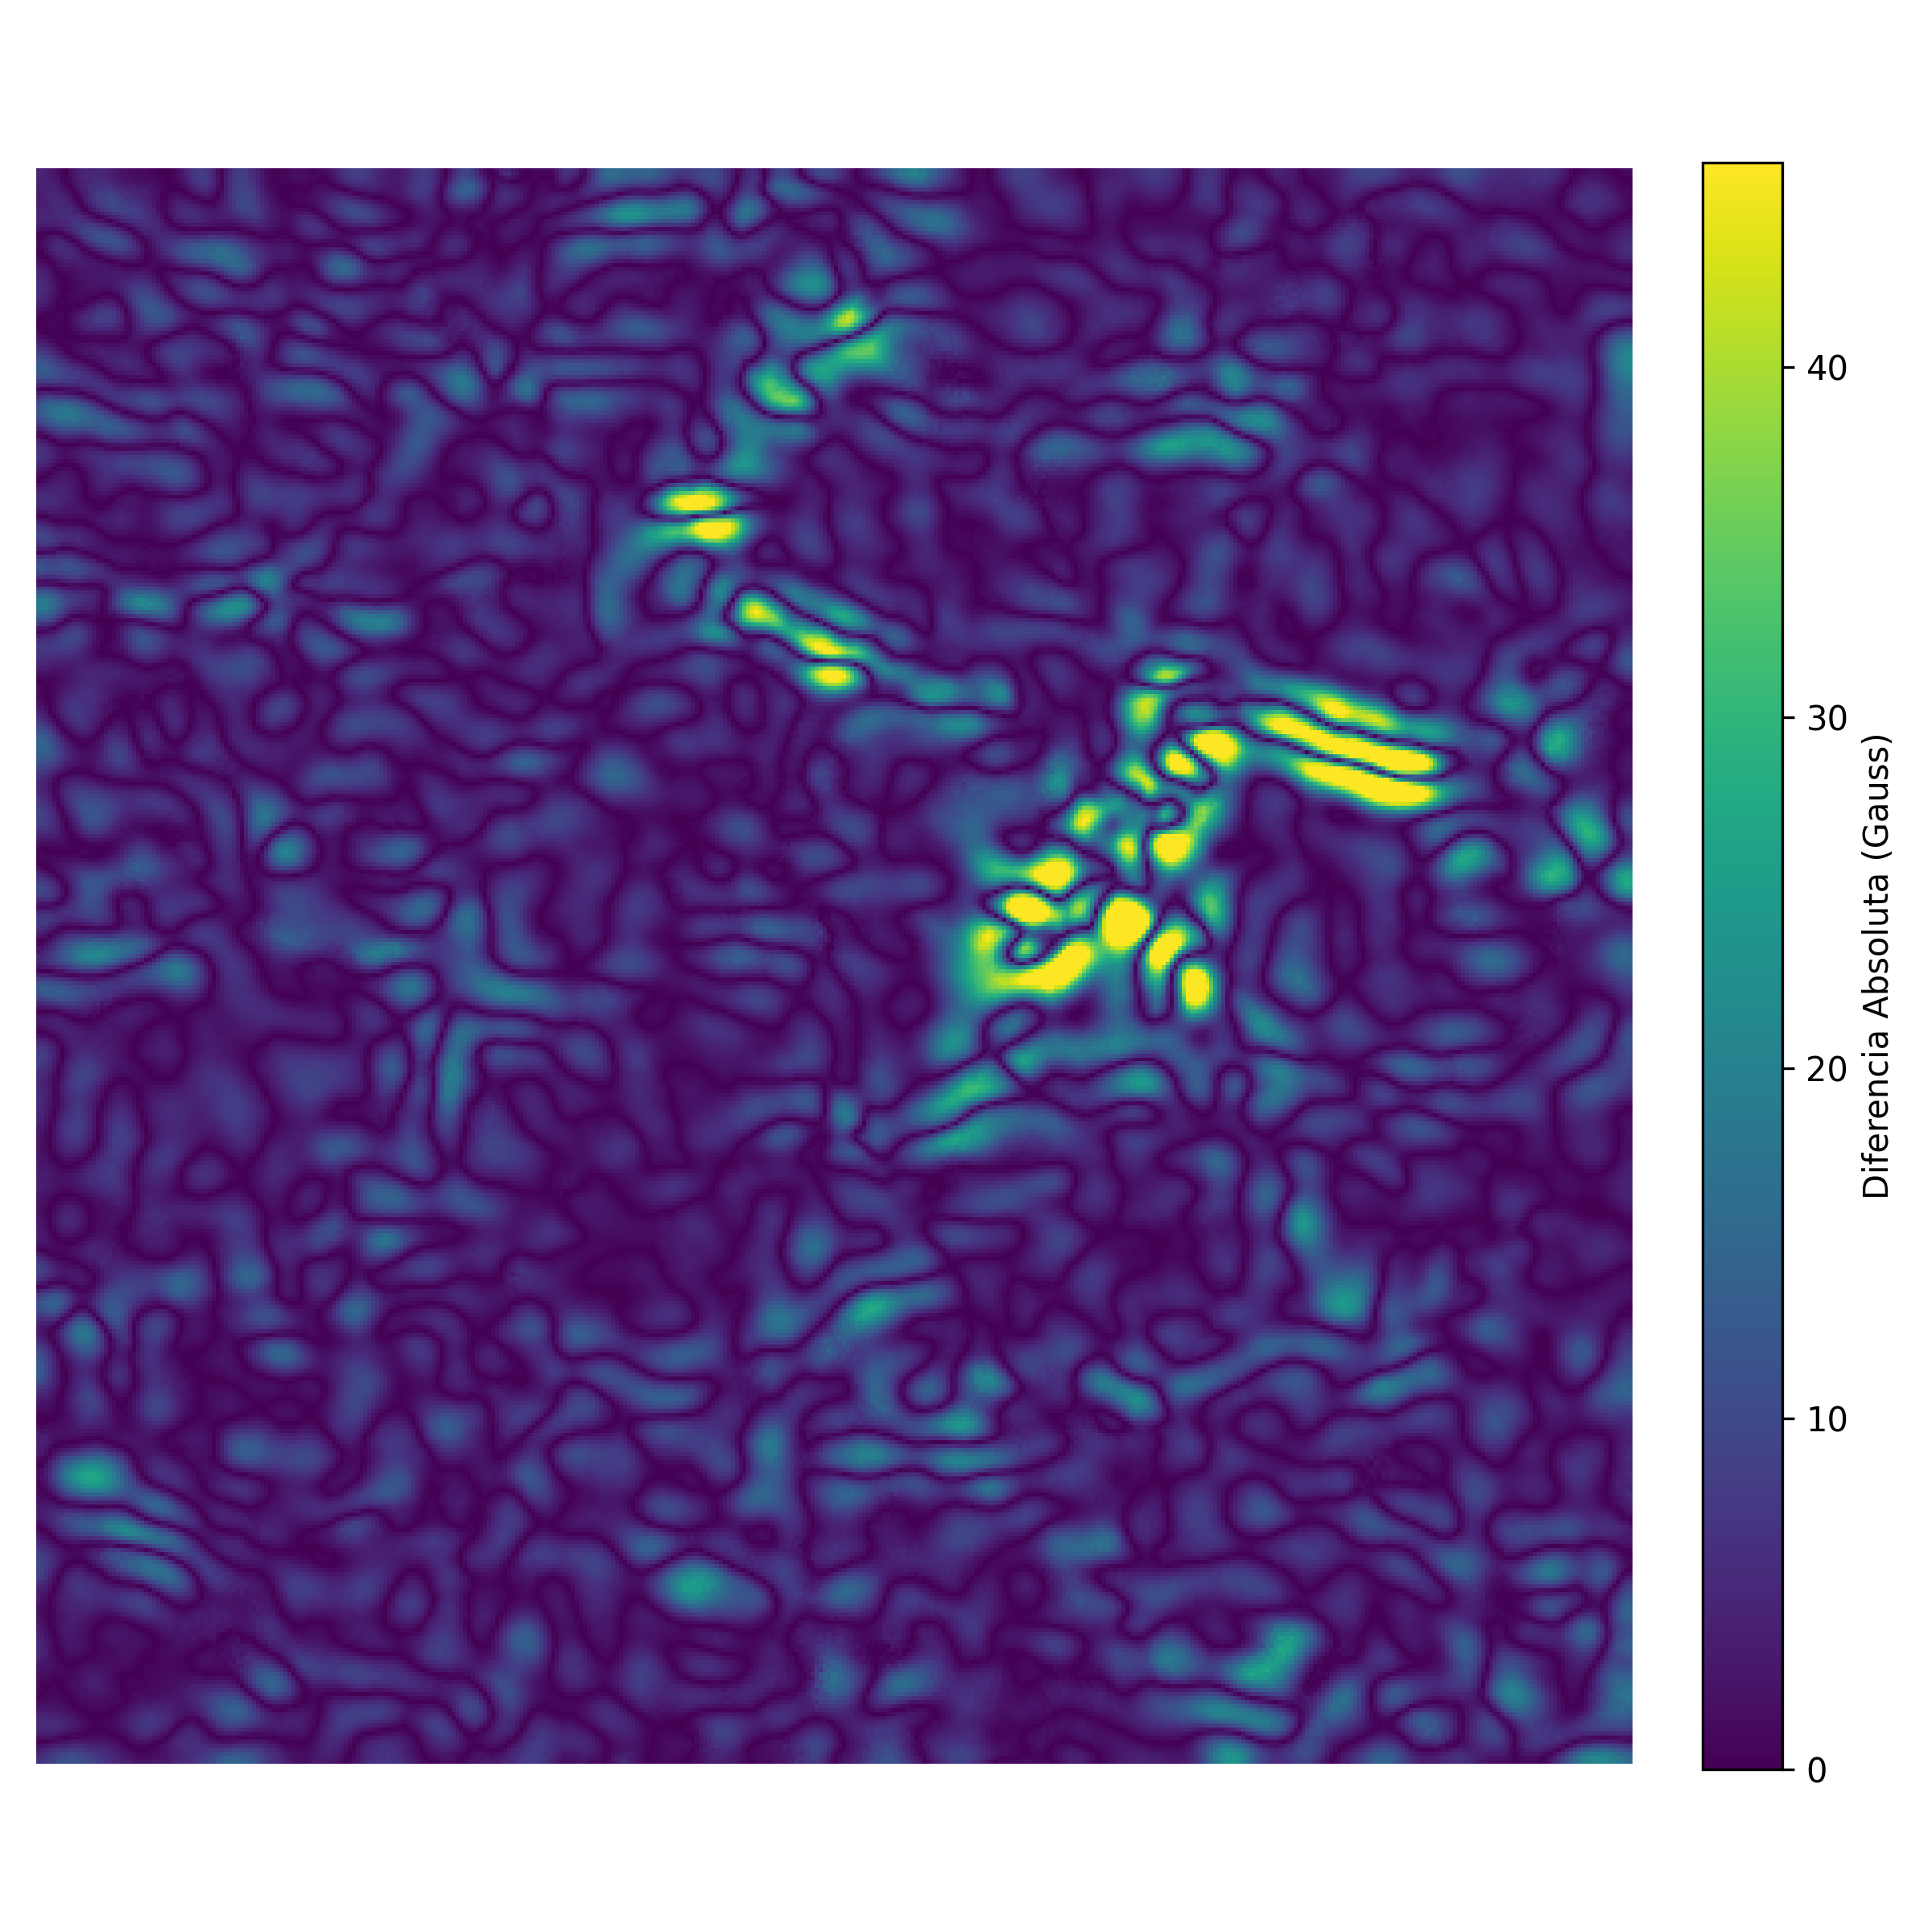
\includegraphics[width=0.9\textwidth]{img/exp4_5_diferencia.png}
    \caption{Mapa de diferencias entre la imagen original y la deconvolucionada del campo magnético, restando las imágenes. Se observa que las diferencias se concentran en las regiones donde el método logra recuperar detalles finos de la estructura del campo magnético.}
    \label{fig:campoMagDecoRealDiferencias}
\end{figure}

Se puede observar que las zonas más brillantes (colores verdes y amarillos) trazan los contornos y fronteras de la estructura magnética, indicando que el algoritmo está reconcentrando el flujo magnético en las zonas que fueron esparcidas por la PSF. 
